\documentclass{article}
\usepackage[utf8]{inputenc}

\usepackage{url}
% For basic math, align, fonts, etc.
\usepackage{amsmath}
\usepackage{amsthm}
\usepackage{amssymb}
\usepackage{mathtools}
\usepackage{mathrsfs}
%\mathtoolsset{showonlyrefs}
\usepackage{graphicx,latexsym, booktabs,array,multirow}
\usepackage{listings}
\usepackage{flexisym}
\usepackage{graphicx}

\usepackage
[
        a4paper,% other options: a3paper, a5paper, etc
        left=2.54cm,
        right=2.54cm,
        top=1.5cm,
        bottom=1.8cm,
        % use vmargin=2cm to make vertical margins equal to 2cm.
        % us  hmargin=3cm to make horizontal margins equal to 3cm.
        % use margin=3cm to make all margins  equal to 3cm.
]{geometry}

\usepackage{hyperref} 

% For color
\usepackage{xcolor}
\definecolor{dark-red}{rgb}{0.4,0.15,0.15}
\definecolor{dark-blue}{rgb}{0,0,0.7}
\hypersetup{
    colorlinks, linkcolor={dark-blue},
    citecolor={dark-blue}, urlcolor={dark-blue}
}

\begin{document}

\begin{center}
    \begin{Large}
    CMPSCI 687 Homework 2
    \end{Large}
    \\
    Submitted By - Ankita Mehta
\end{center}

\section*{Written Portion}
\begin{enumerate}
    \item (10 Points) Apply value iteration to the gridworld used in class (with stochastic state transitions and zero reward for hitting obstacles, as it was originally presented). Remember that $R_t$ is $-10$ if $S_{t+1}$ is the state with water, and $R_t$ is $+10$ if $S_{t+1}$ is the bottom-right state. Begin with the value of every state being zero. Draw the value function as a $5 \times 5$ grid with two cells missing (the obstacles), with numbers in each cell of the grid correspond to the current estimate of the value of that state. After computing $v_{k+1}$, round all values to three decimal places before continuing (your answer should include three decimal places, and future computations should use the rounded values). Show the first ten iterations of value iteration. Below is the initial value function:
    \\\\
    $v_0$:
    \begin{tabular}{|c|c|c|c|c|}
    \hline
        0 & 0 & 0 & 0 & 0\\
        \hline
        0 & 0 & 0 & 0 & 0\\
        \hline
        0 & 0 & N/A & 0 & 0\\
        \hline
        0 & 0 & N/A & 0 & 0\\
        \hline
        0 & 0 & 0 & 0 & 0\\
        \hline
    \end{tabular}
    
    \textbf{Solution:} 1st 10 iterations of value iteration are shown below:
    
    $v_1$:

 \begin{tabular}{|c|c|c|c|c|}

     \hline
      0.000 & 0.000 & 0.000 & 0.000 & 0.000  \\
    \hline
    0.000 & 0.000 & 0.000 & 0.000 & 0.000  \\
    \hline
     0.000 & 0.000 &  N/A & 0.000 & 0.000  \\
    \hline
     0.000 & 0.000 &  N/A & 0.000 & 8.000  \\
    \hline
    0.000 & 0.000 & -2.000 & 8.000 & 0.000  \\
    \hline

\end{tabular} \\\\

$v_2$:

 \begin{tabular}{|c|c|c|c|c|}

     \hline
      0.000 & 0.000 & 0.000 & 0.000 & 0.000  \\
    \hline
    0.000 & 0.000 & 0.000 & 0.000 & 0.000  \\
    \hline
     0.000 & 0.000 &  N/A & 0.000 & 6.400  \\
    \hline
     0.000 & 0.000 &  N/A & 6.800 & 9.200  \\
    \hline
    0.000 & 0.000 & 4.000 & 9.200 & 0.000  \\
    \hline

\end{tabular} \\\\

$v_3$:

 \begin{tabular}{|c|c|c|c|c|}

     \hline
      0.000 & 0.000 & 0.000 & 0.000 & 0.000  \\
    \hline
    0.000 & 0.000 & 0.000 & 0.000 & 5.120  \\
    \hline
     0.000 & 0.000 &  N/A & 5.760 & 8.320  \\
    \hline
     0.000 & 0.000 &  N/A & 8.840 & 9.720  \\
    \hline
    0.000 & 0.000 & 6.160 & 9.720 & 0.000  \\
    \hline

\end{tabular} \\\\

$v_4$:

 \begin{tabular}{|c|c|c|c|c|}

     \hline
      0.000 & 0.000 & 0.000 & 0.000 & 4.096  \\
    \hline
    0.000 & 0.000 & 0.000 & 4.864 & 7.424  \\
    \hline
     0.000 & 0.000 &  N/A & 8.352 & 9.312  \\
    \hline
     0.000 & 0.000 &  N/A & 9.588 & 9.900  \\
    \hline
    0.000 & 0.000 & 7.008 & 9.900 & 0.000  \\
    \hline

\end{tabular} \\\\

$v_5$:

 \begin{tabular}{|c|c|c|c|c|}

     \hline
      0.000 & 0.000 & 0.000 & 4.096 & 6.554  \\
    \hline
    0.000 & 0.000 & 3.891 & 7.539 & 8.806  \\
    \hline
     0.000 & 0.000 &  N/A & 9.389 & 9.734  \\
    \hline
     0.000 & 0.000 &  N/A & 9.853 & 9.964  \\
    \hline
    0.000 & 0.000 & 7.322 & 9.964 & 0.000  \\
    \hline

\end{tabular} \\\\

$v_6$:

 \begin{tabular}{|c|c|c|c|c|}

     \hline
      0.000 & 0.000 & 3.471 & 6.769 & 8.233  \\
    \hline
    0.000 & 3.113 & 6.615 & 8.900 & 9.485  \\
    \hline
     0.000 & 0.000 &  N/A & 9.777 & 9.901  \\
    \hline
     0.000 & 0.000 &  N/A & 9.947 & 9.987  \\
    \hline
    0.000 & 0.000 & 7.436 & 9.987 & 0.000  \\
    \hline

\end{tabular} \\\\

$v_7$:

 \begin{tabular}{|c|c|c|c|c|}

     \hline
      0.000 & 2.932 & 6.267 & 8.382 & 9.161  \\
    \hline
    2.490 & 5.603 & 8.286 & 9.517 & 9.789  \\
    \hline
     0.000 & 2.490 &  N/A & 9.919 & 9.964  \\
    \hline
     0.000 & 0.000 &  N/A & 9.981 & 9.995  \\
    \hline
    0.000 & 0.000 & 7.477 & 9.995 & 0.000  \\
    \hline

\end{tabular} \\\\

$v_8$:

 \begin{tabular}{|c|c|c|c|c|}

     \hline
     2.470 & 5.734 & 8.060 & 9.223 & 9.624  \\
    \hline
    4.731 & 7.460 & 9.170 &  9.791 & 9.915 \\
    \hline
     2.117 & 4.856  & N/A & 9.971 & 9.987 \\
    \hline
     0.000 & 1.992 &  N/A & 9.993 & 9.998 \\
    \hline
    0.000 & 0.000 & 7.491 & 9.998 & 0.000 \\
    \hline

\end{tabular} \\\\

$v_9$:

 \begin{tabular}{|c|c|c|c|c|}

     \hline
     5.194 & 7.681 & 9.046 & 9.639 & 9.837 \\
    \hline
    6.670 & 8.611 & 9.611 & 9.910 & 9.966 \\
    \hline
     4.345 & 6.802 & N/A & 9.989 & 9.995 \\
    \hline
     1.793 & 4.184 & N/A & 9.997 & 9.999 \\
    \hline
    0.000 & 1.468 & 7.497 & 9.999 & 0.000\\
    \hline

\end{tabular} \\\\

$v_{10}$:

 \begin{tabular}{|c|c|c|c|c|}

     \hline
     7.257 & 8.819 & 9.549 & 9.836 & 9.930 \\
    \hline
    8.033 & 9.274 & 9.822 & 9.961 & 9.986\\
    \hline
    6.328 & 8.126 & N/A & 9.996 & 9.998\\
    \hline
     3.954 & 6.159  &  N/A &  9.999 & 10.000 \\
    \hline
    1.508 & 3.369 & 7.499 & 10.000 & 0.000 \\
    \hline

\end{tabular} \\\\

    
    \item (10 Points) Prove that multiplying all rewards (of a finite MDP with bounded rewards) by a positive scalar does not change which policies are optimal, using either of the definitions of optimal policies that we covered in class (that is, show it for at least one of the definitions that we covered in class).
    
    \textbf{Solution:} Let $\pi^*$ be the optimal policy of a finite MDP with bounded rewards , such that there exist $v^{\pi^*}(s) \geq v^{\pi}(s) \forall s \in$ S. \\

   \[v^{\pi}(s) =\mathbb{E}[\sum_{k=0}^{\infty}{\gamma^k R_{t+k} | S_t = s, \pi}]\]	
   
   Given the reward as R of MDP M, let $R_{new} = C*R$ , where C is a positive constant. It has been proved below that multiplying a constant to a reward function doesn't change the optimal policies. 
   
   Taking new R as C*R, $v^{\pi}_{new}(s)$ will be :
   \[v^{\pi}_{new}(s) =\mathbb{E}[\sum_{k=0}^{\infty}{\gamma^k C R_{t+k} | S_t = s, \pi}]\]	
   
   Since, C is a positive constant it can be taken out of expectation.
   
   \begin{align}
   v^{\pi}_{new}(s) &=C*\mathbb{E}[\sum_{k=0}^{\infty}{\gamma^k R_{t+k} | S_t = s, \pi}]  \nonumber \\
			    &=C*v^{\pi}(s)
   \end{align}
   
   Similarly, for $v^{\pi^*}(s)$ , 
   
   \[v^{\pi^*}(s) =\mathbb{E}[\sum_{k=0}^{\infty}{\gamma^k R_{t+k} | S_t = s, \pi^*}]\]	
   
   Taking R_{new} as C*R, $v^{\pi^*}_{new}(s)$ will be :
   \[v^{\pi^*}_{new}(s) =\mathbb{E}[\sum_{k=0}^{\infty}{\gamma^k C R_{t+k} | S_t = s, \pi^*}]\]	
   
   Since, C is a positive constant it can be taken out of expectation.
   
   \begin{align}
   v^{\pi^*}_{new}(s) &=C*\mathbb{E}[\sum_{k=0}^{\infty}{\gamma^k R_{t+k} | S_t = s, \pi^*}] \nonumber \\
			       &=C*v^{\pi^*}(s)
   \end{align}
      
    As we know that $v^{\pi^*}(s) \geq v^{\pi}(s)$ exists for an optimal policy $\pi^*$ and C is a constant, so Using above equations of $v^{\pi}_{new}(s) , v^{\pi^*}_{new}(s)$ , i.e equation 1 and 2, it can be said that $v^{\pi^*}_{new}(s) \geq v^{\pi}_{new}(s)$.
    
    So multiplying reward by a constant doesn't change the optimal policies.
    
    
    \item (5 Points) Prove that adding a positive constant to all rewards (of a finite MDP with bounded rewards) can change which policies are optimal, using either of the definitions of optimal policies that we covered in class.
    
    \textbf{Solution:} Let $\pi^*$ be the optimal policy, such that there exist $v^{\pi^*}(s) \geq v^{\pi}(s) \forall s \in$ S.
    
     Given the reward as R, $R_{new} = R + C$ , where C is a positive constant. Adding a constant to a reward can change the optimal policies. 
     This generally happens, when adding a constant to a reward, can make some negative rewards to positive and then its optimal policy changes accordingly. This can be proved below, by moving in the same manner as above :
     
     \[v^{\pi}(s) =\mathbb{E}[\sum_{k=0}^{\infty}{\gamma^k R_{t+k} | S_t = s, \pi}]\]	
     
     Taking new R as C + R, $v^{\pi}_{new}(s)$ will be :
     \begin{align}
     v^{\pi}_{new}(s) &=\mathbb{E}[\sum_{k=0}^{\infty}{\gamma^k (C + R_{t+k} ) | S_t = s, \pi}] \nonumber \\
     \end{align}
     
     Let's consider an example below: \ref{fig:grid}
    
	\begin{figure}
	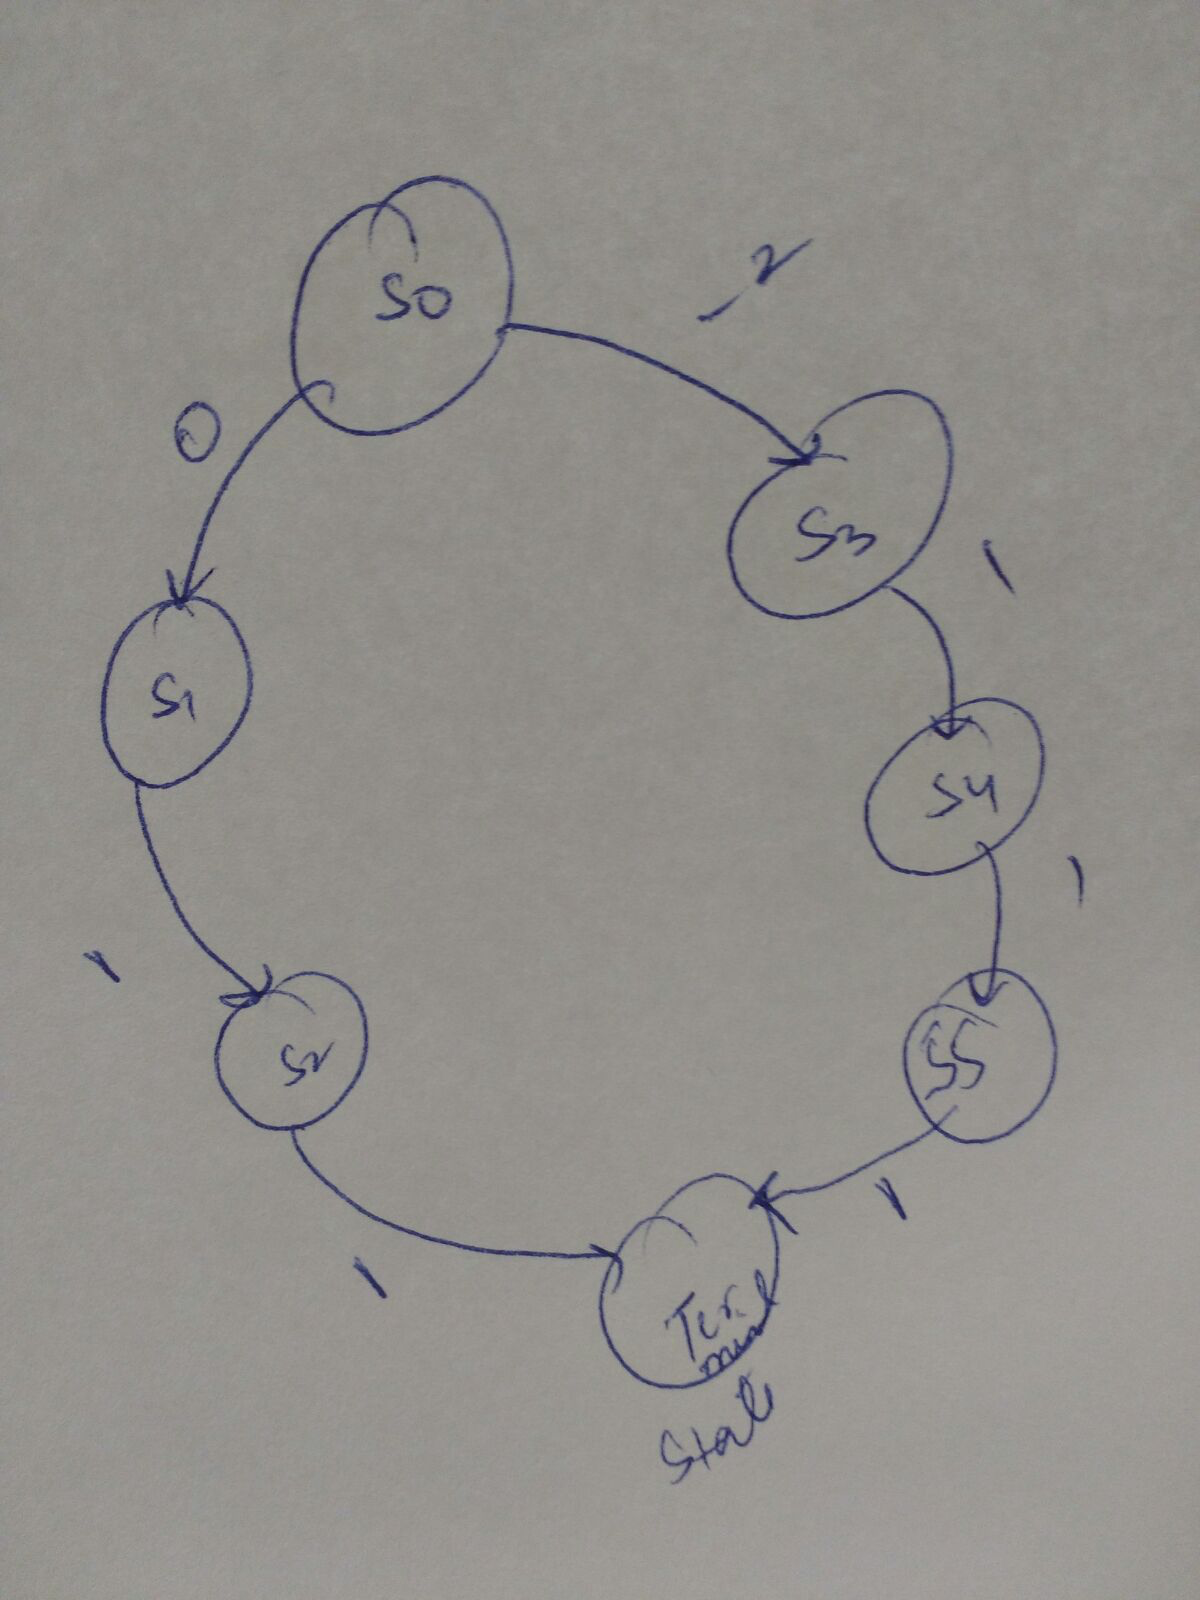
\includegraphics[scale=0.2]{pic}
	\label{fig:grid}
	\end{figure}

	In this example, there are two policies which can be followed at s = $s_0$ which is left and right.   Lets find out $v^{\pi}_{left}, v^{\pi}_{right}, v^{\pi}_{newLeft} , v^{\pi}_{newRight}$ for state $s_0$. Taking $\gamma = 1$
	\[v^{\pi}_{left}(s_0) = 2\]
	\[v^{\pi}_{right}(s_0) = 1\]
	So, optimal policy is the left policy here. \\
	
Now, consider when we add a constant  100 to Reward, then 
\[v^{\pi}_{newLeft}(s_0) = 202\]
\[v^{\pi}_{newRight}(s_0) = 398\]

Now, the optimal policy is right. So, Here adding a constant to the reward has changed the optimal policy.
	
    
    \item (5 Points) Your boss asked you to estimate the state-value function associated with a known policy, $\pi$, for a specific MDP. You misheard and instead estimated the action-value function. This estimation was very expensive, and so you do not want to do it again. Explain how you could easily retrieve the value of any state given what you have already computed.
    
    \textbf{Solution:} Given the policy $\pi$ State value functions can easily be written in form of action value function in the following manner: \\
    
    \[v^{\pi}(s) =\mathbb{E}[\sum_{k=0}^{\infty}{\gamma^k R_{t+k} | S_t = s, \pi}]\]	
    \[q^{\pi}(s) = \mathbb{E}[\sum_{k=0}^{\infty}{\gamma^k R_{t+k} | S_t = s, A_t = a, \pi}]\]
    Marginalising $v^{\pi}(s)$ over action at time t , 
    \[v^{\pi}(s) =\sum_{a}Pr(A_t = a | S_t = s)* \mathbb{E}[\sum_{k=0}^{\infty}{\gamma^k R_{t+k} | S_t = s, A_t = a, \pi}]\]	
    \[v^{\pi}(s) =\sum_{a}\pi(s,a)* \mathbb{E}[\sum_{k=0}^{\infty}{\gamma^k R_{t+k} | S_t = s, A_t = a, \pi}]\]	
        \[v^{\pi}(s) =\sum_{a}\pi(s,a)* q^{\pi}(s,a)\]
    
    \item (10 Points) Consider a finite MDP with bounded rewards, where all rewards are negative. That is, $R_t < 0$ always. Let $\gamma=1$. The MDP is finite horizon, with horizon $L$, and also has a deterministic transition function and initial state distribution (rewards may be stochastic). Let $H=(S_0,A_0,R_0,S_1,A_2,R_1,\dotsc,S_{L-1},A_{L-1},R_{L-1})$ be any history that can be generated by a deterministic policy, $\pi$. Prove that the sequence $v^\pi(S_0), v^\pi(S_1),\dotsc,v^\pi(S_{L-1})$ is strictly increasing.
    \textbf{Solution:} Using the bellman equation for state value function:
        
     \[v^{\pi}(S_i) =\sum_{a} \pi(S_i,a) \sum_{S_{i+1} \in S} P(S_i , a, S_{i+1}) ( R(S_i , a , S_{i+1}) + \gamma v^{\pi}(S_{i+1}))\]
     
     It is given that $\gamma = 1$ , state transition function and policy $\pi$ are deterministic, \\ so $\sum_{a} \pi(S_i,a) , \gamma ,  \sum_{S_{i+1} \in S} P(S_i , a, S_{i+1})$ can we written as 1.\\
     
     So, the bellman equation will become : 
     
     \[v^{\pi}(S_i) = R(S_i , a , S_{i+1}) + v^{\pi}(S_{i+1})\]
     
     Now, since R is negative , so $v^{\pi}(S_i) \leq v^{\pi}(S_{i+1}) $. So the sequence $v^\pi(S_0), v^\pi(S_1),\dotsc,v^\pi(S_{L-1})$ is strictly increasing.
    
    \item (15 Points) The Bellman operator for $q$-functions is:
    $$
    \mathcal T:\mathcal q \to \mathcal q,
    $$
    where $\mathcal Q$ is the set of all functions, $q:\mathcal S \times \mathcal A \to \mathbb R$ and
    $$
    Tq(s,a)\coloneqq \sum_{s'}P(s,a,s')\left ( R(s,a,s') + \gamma \max_{a'} q(s',a')\right ).
    $$
    Prove that the Bellman operator for $q$-functions is a contraction mapping.
    
    \textbf{Solution:} To prove that Bellman operator for $q$ -functions is a contraction mapping, we need to prove that $||Tq - Tq'|| \leq \lambda ||q - q'||$
    
    \textbf{Proof:} \\
    \begin{align}    
    ||Tq - Tq'|| &= \max_{s,a} | Tq(s,a) - Tq'(s,a) | \nonumber \\
    		    &=\max_{s,a} | \sum_{s'}P(s,a,s')\left ( R(s,a,s') + \gamma \max_{a'} q(s',a')\right ) - \sum_{s'}P(s,a,s')\left ( R(s,a,s') + \gamma \max_{a'} q'(s',a')\right )| \nonumber \\
		    &=\max_{s,a} | \sum_{s'}P(s,a,s') \gamma \max_{a'} q(s',a') - \sum_{s'}P(s,a,s') \gamma \max_{a'} q'(s',a') | \nonumber\\
		    &=\gamma\max_{s,a} | \sum_{s'}P(s,a,s') \max_{a'} q(s',a') - \sum_{s'}P(s,a,s') \max_{a'} q'(s',a') | \nonumber\\
		    &=\gamma\max_{s,a} | \sum_{s'}P(s,a,s') \left (\max_{a'} q(s',a') - \max_{a'} q'(s',a') \right )| \nonumber\\
		    &\leq \gamma\max_{s,a}\max_{a'} | \sum_{s'}P(s,a,s') \left ( q(s',a') - q'(s',a') \right )| \nonumber\\
		    &\leq \gamma\max_{s,a}\max_{a'} \max_{s'} |q(s',a') - q'(s',a')| \nonumber\\ 
		    &\leq \gamma \max_{a'} \max_{s'} |q(s',a') - q'(s',a')| \tag{Removing max over s,a} \nonumber\\
		    &\leq \gamma ||q - q'|| \tag{By Using max norm} \\
    \end{align}
    
    Hence, $q$ -value functions is a contraction mapping.
    \item (10 Points) A researcher proposes an estimator, $\hat J$, of $J$. The estimator uses data to estimate the performance of a policy. That is, $\hat J(\pi,H)$ corresponds to the estimator's estimate of $J(\pi)$, where $H$ is a history produced by running $\pi$ for one episode. Specifically:
    $$
    \hat J(\pi,H) = \sum_{t=0}^\infty \gamma^t \left ( R_t - R(S_t,A_t,S_{t+1})\right ) + \sum_{t=0}^\infty \gamma^t \sum_{s'} P(S_t,A_t,s')R(S_t,A_t,s').
    $$
    Now consider the case where we have a data set, $D_n$, that includes $n \in \mathbb N_{>0}$ i.i.d.~histories, i.e., $D_n=(H_1,\dotsc,H_n)$, each produced by running the policy $\pi$. We construct a new estimator, $\hat J_n(\pi,D_n)=\frac{1}{n}\sum_{i=1}^n \hat J(\pi,H_i)$. Prove that $\hat J_n(\pi,D_n)$ converges in probability to $J(\pi)$. That is, for all $\epsilon$,
    $$
    \lim_{n\to\infty} \Pr \left ( | \hat J_n(\pi,D_n) - J(\pi) | > \epsilon \right ) = 0.
    $$
\end{enumerate}
\textbf{Solution:}  Using  weak law of large numbers , if we prove that $\mathbb E(\hat J(\pi,H_i))  = J(\pi)$ , \\
that means $\lim_{n\to\infty} \Pr \left ( | \hat J_n(\pi,D_n) - J(\pi) | > \epsilon \right ) = 0.$ \\

\[\hat J(\pi,H) = \sum_{t=0}^\infty \gamma^t \left ( R_t - R(S_t,A_t,S_{t+1})\right ) + \sum_{t=0}^\infty \gamma^t \sum_{s'} P(S_t,A_t,s')R(S_t,A_t,s').\]

\begin{align}
\mathbb E(\hat J(\pi,H)) &= \mathbb E(\sum_{t=0}^\infty \gamma^t \left ( R_t - R(S_t,A_t,S_{t+1})\right ) + \sum_{t=0}^\infty \gamma^t \sum_{s'} P(S_t,A_t,s')R(S_t,A_t,s')) \nonumber\\
				     &= \mathbb E(\sum_{t=0}^\infty \gamma^t ( R_t ) - \mathbb E(\sum_{t=0}^\infty \gamma^t R(S_t,A_t,S_{t+1}) + \mathbb E(\sum_{t=0}^\infty \gamma^t \sum_{s'} P(S_t,A_t,s')R(S_t,A_t,s')) \nonumber\\
				     &= J(\pi) + - \mathbb E(\sum_{t=0}^\infty \gamma^t R(S_t,A_t,S_{t+1}) + \mathbb E(\sum_{t=0}^\infty \gamma^t \sum_{s'} P(S_t,A_t,s')R(S_t,A_t,s')) \nonumber\\
				     &= J(\pi) + - \mathbb E(\sum_{t=0}^\infty \gamma^t R(S_t,A_t,S_{t+1})) + \sum_{t=0}^\infty \gamma^t \sum_{s'} P(S_t,A_t,s')R(S_t,A_t,s') \tag{expectation of a constant is a constant} \nonumber\\
				     &= J(\pi) + - \sum_{t=0}^\infty \gamma^t \mathbb E(R(S_t,A_t,S_{t+1})) + \sum_{t=0}^\infty \gamma^t \sum_{s'} P(S_t,A_t,s')R(S_t,A_t,s') \tag{expectation of a constant is a constant}\\
\end{align}

Considering, $S_{t+1} $as a random variable, and $ \mathbb E [g(X)] = \sum_{x \in X}g(x) f(x) $

\begin{align}
\mathbb E(R(S_t,A_t,S_{t+1})) &= \sum_{S_{t+1}} P(S_t,A_t,S_{t+1})R(S_t,A_t,S_{t+1}) \nonumber\\
							    &= \sum_{s'} P(S_t,A_t,s)R(S_t,A_t,s')
\end{align}

After putting equation 6 into 5, we can say that $ \mathbb E(\hat J(\pi,H)) = J(\pi). $
\end{document}
